\documentclass[letterpaper,12pt]{article}
\usepackage{array}
\usepackage{threeparttable}
\usepackage{geometry}
\geometry{letterpaper,tmargin=1in,bmargin=1in,lmargin=1.25in,rmargin=1.25in}
\usepackage{fancyhdr,lastpage}
\pagestyle{fancy}
\lhead{}
\chead{}
\rhead{}
\lfoot{}
\cfoot{}
\rfoot{\footnotesize\textsl{Page \thepage\ of \pageref{LastPage}}}
\renewcommand\headrulewidth{0pt}
\renewcommand\footrulewidth{0pt}
\usepackage[format=hang,font=normalsize,labelfont=bf]{caption}
\usepackage{listings}
\lstset{frame=single,
  language=Python,
  showstringspaces=false,
  columns=flexible,
  basicstyle={\small\ttfamily},
  numbers=none,
  breaklines=true,
  breakatwhitespace=true
  tabsize=3
}
\usepackage{amsmath}
\usepackage{amssymb}
\usepackage{amsthm}
\usepackage{harvard}
\usepackage{setspace}
\usepackage{float,color}
\usepackage[pdftex]{graphicx}
\usepackage{hyperref}
\hypersetup{colorlinks,linkcolor=red,urlcolor=blue}
\theoremstyle{definition}
\newtheorem{theorem}{Theorem}
\newtheorem{acknowledgement}[theorem]{Acknowledgement}
\newtheorem{algorithm}[theorem]{Algorithm}
\newtheorem{axiom}[theorem]{Axiom}
\newtheorem{case}[theorem]{Case}
\newtheorem{claim}[theorem]{Claim}
\newtheorem{conclusion}[theorem]{Conclusion}
\newtheorem{condition}[theorem]{Condition}
\newtheorem{conjecture}[theorem]{Conjecture}
\newtheorem{corollary}[theorem]{Corollary}
\newtheorem{criterion}[theorem]{Criterion}
\newtheorem{definition}[theorem]{Definition}
\newtheorem{derivation}{Derivation} % Number derivations on their own
\newtheorem{example}[theorem]{Example}
\newtheorem{exercise}[theorem]{Exercise}
\newtheorem{lemma}[theorem]{Lemma}
\newtheorem{notation}[theorem]{Notation}
\newtheorem{problem}[theorem]{Problem}
\newtheorem{proposition}{Proposition} % Number propositions on their own
\newtheorem{remark}[theorem]{Remark}
\newtheorem{solution}[theorem]{Solution}
\newtheorem{summary}[theorem]{Summary}
%\numberwithin{equation}{section}
\bibliographystyle{aer}
\newcommand\ve{\varepsilon}
\newcommand\boldline{\arrayrulewidth{1pt}\hline}


\begin{document}

\begin{flushleft}
  \textbf{\large{Problem Set \#2}} \\
  MACS 30000, Dr. Evans \\
  Xingyun Wu
\end{flushleft}

\vspace{5mm}

\noindent\textbf{Problem 1: Some income data, lognormal distribution, and hypothesis testing}

\vspace{2mm}

\textbf{Part (a).} The histogram is shown in Figure 1.
\begin{figure}[htb]\centering\captionsetup{width=4.0in}
  \caption{\textbf{Histogram of Percentages of the MACSS Graduates}}\label{Fig1a}
  \fbox{\resizebox{4.0in}{3.0in}{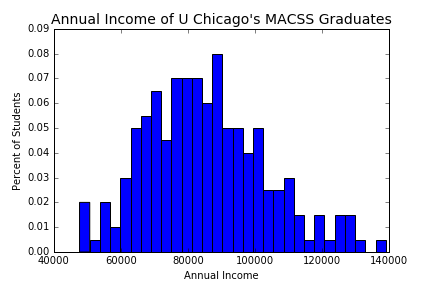
\includegraphics{Fig_1a.png}}}
\end{figure}

\textbf{Part (b).} The log likelihood value is approximately: -8298.64. The plot of lognormal PDF is shown in Figure 2.
\begin{figure}[htb]\centering\captionsetup{width=4.0in}
  \caption{\textbf{Lognormal PDF}}\label{Fig1b}
  \fbox{\resizebox{4.0in}{3.0in}{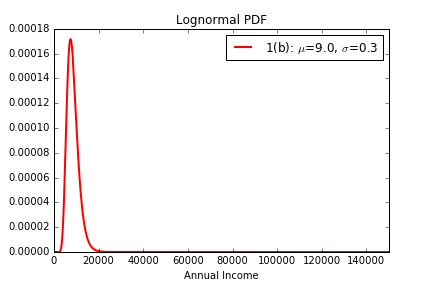
\includegraphics{Fig_1b.png}}}
\end{figure}

\vspace{2mm}

\textbf{Part (c).} The PDF of lognormal distribution by maximum likelihood against the PDF from part(b) and the histogram from part(a) is in Figure 3.\\
ML estimate for mu is approximately: 11.33\\
ML estimate for sigma is approximately: 0.21\\
The value of the likelihood function is approximately: -2239.55\\

\begin{figure}[htb]\centering\captionsetup{width=4.0in}
  \caption{\textbf{Lognormal PDF}}\label{Fig1c}
  \fbox{\resizebox{4.0in}{3.0in}{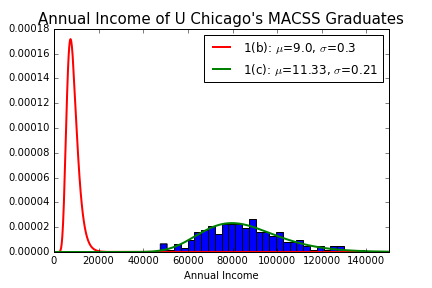
\includegraphics{Fig_1c.png}}}
\end{figure}

\textbf{Part (d).} Chi squared of null-hypothesis (H0) with 2 degrees of freedom =  0.0000. This means we could reject the hypothesis that the model in part(b) fits the data.
The variance-covariance matrix is:
\begin{bmatrix}
0.00030507 &  0.00018687\\
0.00018687  & 0.00054403\\
\end{bmatrix}

\vspace{2mm}

\textbf{Part (e).} The probability of earning more than \$100,000 is approximately:  0.1919. The probability of earning less than \$75,000 is approximately:  0.3089

\vspace{5mm}

\noindent\textbf{Problem 2: Linear regression and MLE}

\vspace{2mm}

\textbf{Part (a).} The parameters of the model by maximum likelihood are approximately:
\begin{align*}
 \sigma_{MLE} &= 0.00302, 
 \beta_0 = 0.25160, 
 \beta_1 = 0.01293, 
 \beta_2 = 0.40053, 
 \beta_3 = -0.00999
\end{align*}
\\
The value of the likelihood function is approximately: 872.18
The estimated variance covariance matrix is:
\begin{bmatrix}
1. & 0. & 0. & 0. & 0.\\
0. & 1. & 0. & 0. & 0.\\
0. & 0. & 1. & 0. & 0.\\
0. & 0. & 0. & 1. & 0.\\
0. & 0. & 0. & 0. & 1.\\
\end{bmatrix}

\textbf{Part (b).} The parameters of null-hypothesis are:\\
\begin{align*}
 H_0: 
 \sigma^{2} = 0.01, 
 \beta_0 = 1, 
 \beta_1 = 0, 
 \beta_2 = 0, 
 \beta_3 = 0
\end{align*}
\\
Chi squared of H0 with 2 degrees of freedom =  0.0000, which means we could reject the null-hypothesis that the variables of age, number of children, and average temperature in winter have no impact on sickness.

\vspace{5mm}

\textbf{Please see the next page for Figure 3, Problem 1(c).}

\end{document}

